%%%%%%%% ICML 2021 EXAMPLE LATEX SUBMISSION FILE %%%%%%%%%%%%%%%%%

\documentclass{article}

% Recommended, but optional, packages for figures and better typesetting:
\usepackage{microtype}
\usepackage{graphicx}
\usepackage{subfigure}
\usepackage{booktabs} % for professional tables

% hyperref makes hyperlinks in the resulting PDF.
% If your build breaks (sometimes temporarily if a hyperlink spans a page)
% please comment out the following usepackage line and replace
% \usepackage{icml2021} with \usepackage[nohyperref]{icml2021} above.
\usepackage{hyperref}

% Attempt to make hyperref and algorithmic work together better:
\newcommand{\theHalgorithm}{\arabic{algorithm}}

% Use the following line for the initial blind version submitted for review:
\usepackage{icml2021}
\usepackage{natbib}

% If accepted, instead use the following line for the camera-ready submission:
%\usepackage[accepted]{icml2021}

% The \icmltitle you define below is probably too long as a header.
% Therefore, a short form for the running title is supplied here:
\icmltitlerunning{Decoding the Neural Correlates of Decision Speed in Speech Perception using CNNs}

\begin{document}

\twocolumn[
\icmltitle{Decoding the Neural Correlates of Decision Speed in Speech Perception using CNNs}

% It is OKAY to include author information, even for blind
% submissions: the style file will automatically remove it for you
% unless you've provided the [accepted] option to the icml2021
% package.

% List of affiliations: The first argument should be a (short)
% identifier you will use later to specify author affiliations
% Academic affiliations should list Department, University, City, Region, Country
% Industry affiliations should list Company, City, Region, Country

% You can specify symbols, otherwise they are numbered in order.
% Ideally, you should not use this facility. Affiliations will be numbered
% in order of appearance and this is the preferred way.
\icmlsetsymbol{equal}{*}

\begin{icmlauthorlist}
\icmlauthor{Aeiau Zzzz}{equal,to}
\icmlauthor{Bauiu C.~Yyyy}{equal,to,goo}
\icmlauthor{Cieua Vvvvv}{goo}
\icmlauthor{Iaesut Saoeu}{ed}
\icmlauthor{Fiuea Rrrr}{to}
\icmlauthor{Tateu H.~Yasehe}{ed,to,goo}
\icmlauthor{Aaoeu Iasoh}{goo}
\icmlauthor{Buiui Eueu}{ed}
\icmlauthor{Aeuia Zzzz}{ed}
\icmlauthor{Bieea C.~Yyyy}{to,goo}
\icmlauthor{Teoau Xxxx}{ed}
\icmlauthor{Eee Pppp}{ed}
\end{icmlauthorlist}

\icmlaffiliation{to}{Department of Computation, University of Torontoland, Torontoland, Canada}
\icmlaffiliation{goo}{Googol ShallowMind, New London, Michigan, USA}
\icmlaffiliation{ed}{School of Computation, University of Edenborrow, Edenborrow, United Kingdom}

\icmlcorrespondingauthor{Cieua Vvvvv}{c.vvvvv@googol.com}
\icmlcorrespondingauthor{Eee Pppp}{ep@eden.co.uk}

% You may provide any keywords that you
% find helpful for describing your paper; these are used to populate
% the "keywords" metadata in the PDF but will not be shown in the document
\icmlkeywords{Machine Learning, ICML}

\vskip 0.3in
]

% this must go after the closing bracket ] following \twocolumn[ ...

% This command actually creates the footnote in the first column
% listing the affiliations and the copyright notice.
% The command takes one argument, which is text to display at the start of the footnote.
% The \icmlEqualContribution command is standard text for equal contribution.
% Remove it (just {}) if you do not need this facility.

%\printAffiliationsAndNotice{}  % leave blank if no need to mention equal contribution
\printAffiliationsAndNotice{\icmlEqualContribution} % otherwise use the standard text.

\begin{abstract}
Categorical perception (CP) is a cognitive process of grouping speech sounds into distinct categories.
Decision speed in CP tasks reflects the perceptual difficulty of auditory stimuli and is captured by
the listener's response time (RT). The cognitive processes involved in mapping neural activities
to behavioral RT are subject to individual variations. This paper presents a data-driven approach
and develops parameter-optimized models to understand the relationship between cognitive events
and behavioral response (e.g., RT) of individuals. To investigate the neural correlates of
decision speed in speech categorization, we have explored convolutional neural networks (CNN) to
learn and decode CP behavior from EEG recordings. We applied GradCAM to gain insight into the
learned representation of the CNN models and infer the neural orientation underlying CP behavior.
We further show that activation values from Guided-GradCAM outputs can quantify learned representation
of CNNs as analysis of them reveals neural patterns consistent with prior findings of CP behavior.
\end{abstract}

\section{Introduction}
\label{submission}

Categorical perception (CP) of speech is a cognitive process of grouping sounds into small phonetic categories \cite{cp}. CP is critical in understanding the neural process of speech comprehension and learning. It is an effect that is found to be present in infants and evolves due to speech training \cite{infant_cp}. Thus, investigating the neural organization of CP provides insight into the neural process of speech perception from an elementary level. The lexical processing paradigm of CP is well studied; however, the neural orientation of speech perception, which induces variation in individuals' decision speed, is obscure. In CP studies, the response time (RT) is captured by measuring the time lapse between the voice onset time (VOT) and the time of the actual response (need to cite). RTS effectively capture the decision speed of listeners \cite{decisionspeed} and analysis of RTs can reveal the cause of perceptual difference between subjects. Investigating the neural correlates of decision speed in speech categorization can also explain the variation in behavior across and within-subjects.

The cognitive processes involved in mapping neural activities to behavioral responses can be decoded through in-depth analysis of neurophysiological recordings such as EEG. Decoding categorical perception (CP) from EEG recordings involves analyzing spatial-spectral-temporal properties that define the underlying cognitive functions \cite{beta2, Mahmud_2, Mahmud2019}. The spatial, spectral, and temporal aspects explain \emph{'where'} in the brain, the type of operation (i.e., memory, attention) and  \emph{'when'} in time the neural activities occurs. While hypothesis-driven analysis is being widely used in decoding properties of CP, the multivariate approach based on machine learning (ML) algorithms have been gaining momentum. For example, the ML-based approach reported in \cite{Mahmud2019, Mahmud_2} show promising results in determining contributing factors in age-related hearing loss. Another work reported in \cite{Al_Fahad_2020} used an ML-based approach to decode functional connectivity patterns in CP. The mentioned studies uses classical ML, such as support vector machines (SVM) \cite{svm} with stability selections \cite{stability_selection} to model cognitive processes involved in CP. The feature selection process using stability selection provides a limited interpretation of the causal relationship between neural activities and behavioral responses.

To capture the relationship between cognitive events and behavioral responses (e.g., RT), we present a deep learning approach to first learn the underlying cognitive function and then infer the neural process of CP behavior from learned representations. Inferring regional or spatial orientation of cognitive processes from EEG recordings is difficult due to low spatial resolution and noise. To learn the spatial organization from EEG data, 1) it is required to have a spatial representation extracted from EEG signals, 2) and a robust noise reduction technique. To this extent, we have utilized band power topomaps to represent the spatial contents from EEG data and a bootstrap averaging process to reduce noise in EEG signals. We randomly sample trials (with replacement) within a subject's RT category and average them to generate event-related potentials (ERP). ERPs contain less noise than the original EEG signals due to averaging of multiple trials. We then compute those ERPs' band powers and project them into a 2D topographic representation of the scalp surface known as topomaps. The bandpower topographical representation is introduced by \cite{bashivan2015} and captures the spatial-temporal-spectral contents from EEG signals. However, in our work, we have focused on the spatial-spectral representation since we want to decode the neural organization of CP rather than the temporal aspect.

We introduce convolutional neural networks (CNN) to learn the spatial-spectral representation from EEG recordings. CNNs have been successful in computer vision tasks and have proven capacity in learning spatial representations. CNNs have also been successful in modeling neural processes from EEG data. \cite{bci_mi4, bci_mi6, bci_mi7} used different CNN models to achieve significant results in modeling MI tasks from EEG data. \cite{bci_mi5, bci_mi2} combined CNNs with stacked and variational autoencoders to predict limb movements from EEG recordings. \cite{bashivan2015} was one of the early application of DL in cognitive neuroscience where the cognitive load was modeled using recurrent convolution neural network (RCNN) from spatial-spectral-temporal features extracted from EEG. \cite{mw1} designed channel-wise convolution neural networks (CCNN) and CNN with Restricted Boltzmann Machine (CCNN-R) to model drivers' cognitive state from EEG data. \cite{bci_mi5, bci_mi2} combined CNNs with stacked and variational autoencoders to predict limb movements from EEG recordings. Inspired by these applications, we chose CNNs to learn the neural processes underlying speech categorization behavior.

To capture the general neural patterns of different CP behavior, we have chosen to form the problem irrespective of population. We have defined three RT classes (slow, medium, and fast), which is irrespective of population, i.e., the RT categories are formed using individual trials rather than subjects. To form RT categories, we apply Gaussian Mixture Model (GMM) clustering in the RTs of all available trials. The bootstrap and averaging process for generating ERPs are carried out within each RT class of a subject and converted to band power topomaps. We chose to represent the spatial orientation of $\alpha, \beta$ and $\gamma$ frequency bands in the topomaps as they are highly correlated with CP \cite{alpha, beta1, net_gamma1}. We train CNNs using these band power topomaps to learn the representation of these different RT categories. We deploy the Bayesian hyperparameter optimization algorithm, the tree-structured Parzen Estimator (TPE) \cite{TPE_1} to find the best configuration for our CNN model. Finally, we use our best performing model to interpret the neural process of CP behavior from learned representation.

In deep learning (DL), model interpretation is still a challenge as these models contain millions of parameters and therefore are difficult to interpret. Visual interpretations are the only effective ways to get an insight into the learned features of a neural model. The visual interpretation of models are achieved through class discriminative feature visualization techniques like class activation maps \cite{CAM}, GradCAM \cite{gradcam}, CNN-fixation \cite{cnn_fixation} and EigenCAM \cite{EigenCAM}. Studies like \cite{eeg_cnn_gradcam, eeg_cnn_gradcam2, eeg_cnn_gradcam3} shows that GradCAM does capture feature importance allocation by CNNs from EEG data and therefore could be used to infer spatial-spectral-temporal properties underlying a cognitive event. Despite the successes in visual interpretations, we acknowledge that it is impossible to infer any neural process using these visualizations alone. It is required to quantify the learned representations of neural models to infer any cognitive process from them. We have used activation values from Guided-GradCAM outputs to quantify the learned representation of our CNN models to address this issue. We analyze these activation values to explain the neural correlates of decision speed in speech categorization.

We empirically evaluate the CNN models using the CP data obtained from 50 participants. Our analysis using the activation values shows that the right frontal regions are crucial in determining listeners' decision speed. We also find that all three bands ($\alpha, \beta, \gamma$) have active and passive roles, while the $\gamma$ band is the most significant in driving listeners' RT. The significance of the $\gamma$ band suggests that auditory CP ability in individuals is the primary predictor of their decision speed. Our findings are coherent with recent and prior studies of brain-behavior function in auditory CP, a validation of our decoding process using CNNs.


\section{Data}

\textbf{Participants:} The dataset consisted of 50 participants, which we used for modeling the behavioral aspect of CP. All of the participants were recruited from the University of Memphis student body and the Greater Memphis area. The experiment consisted of 15 males and 35 females aging between 18 and 60 years with a mean of $\approx$ 24. Participants were strongly right-handed (mean Edinburgh Hand Score $\approx$ 80.0), had acquired a collegiate level of education (mean $\approx$ 17 years), and had a median of 1 year of formal music training. All participants were paid for their time and gave informed consent in compliance with the Institutional Review Board at the University of Memphis. Figure \ref{demograph} (A, B) shows the demographic of the participants.

\begin{figure}[ht]
\vskip 0.2in
\begin{center}
\centerline{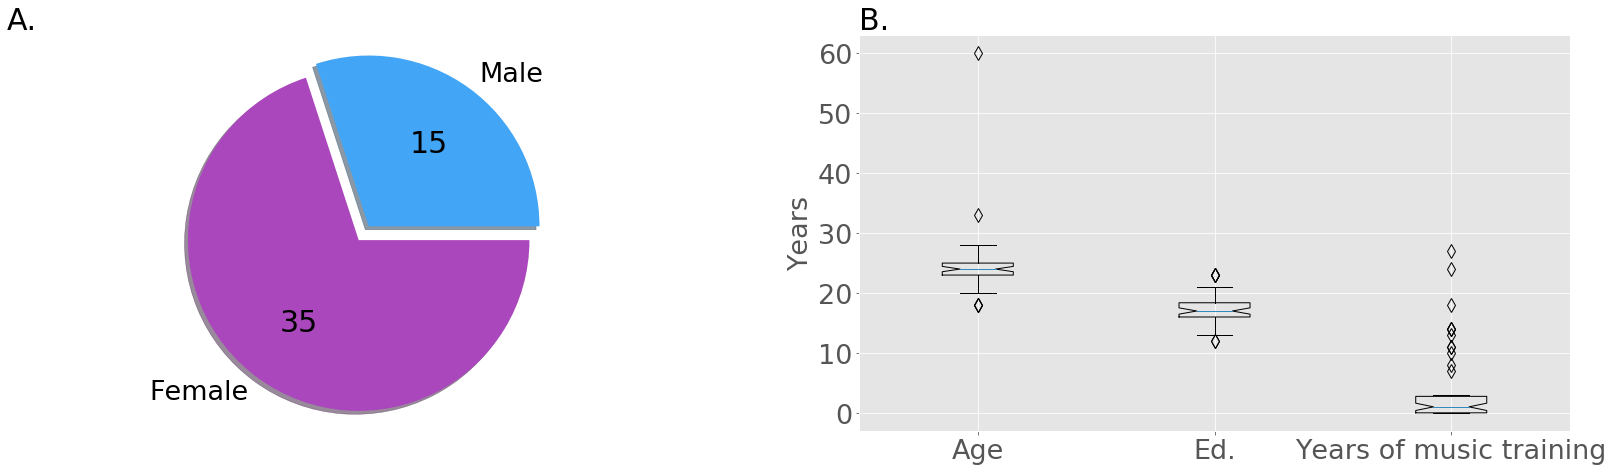
\includegraphics[width=\columnwidth]{Images/demograph}}
\caption[Demographic Information]{A) Gender distribution B) Demography of the participants (includes age, musical training, and education)}
\label{topomap_gen}
\end{center}
\vskip -0.2in
\end{figure}

\textbf{EEG Recording \& Preprocessing:} During the experiment, the participants were instructed to listen from a five-step vowel continuum; each token of the continuum was separated by equidistant steps based on first formant frequency (F1) categorically perceived as /u/ to /a/. Tokens were 100 ms long, including 10 ms rise and fall time. The stimuli were delivered through shielded insert earphones; listeners heard 150-200 trials of individual tokens and were asked to label the sound as perceived through binary responses (‘u’ or ‘a’). Response times (RTs) were recorded as the difference between the stimulus onset and the behavioral response (labeling of tokens). Simultaneous EEG recording was carried out using 64 sintered Ag/AgCI electrodes at standard 10-10 locations around the scalp during the trials. As subsequent preprocessing steps, ocular artifacts were corrected using principal component analysis (PCA), filtered (bandpass: 1-100 Hz; notch filter: 60 Hz), epoched (-200 to 800 ms) into single trials, and baseline corrected (-200 ms to 0 ms).

\textbf{Clustering RTs:} To learn behavioral CP, we opted to form categories within RTs from all the samples using the exact process in \cite{Al_Fahad_2020}. The idea is to use Gaussian Mixture Model (GMM) with expectation-maximization (EM) to identify the plausible number of clusters from the distribution of RTs. We found four clusters within the distribution of RT using the Bayesian Information Criterion (BIC) as a metric to select the optimal number of components (clusters, ranges from 1-14) and the type of covariance parameter (full, tied, diagonal, and spherical). The procedure concluded with an optimal of four clusters using covariance type ‘spherical.’ We inferred fast, medium, and slow RTs as the underlying categories based on the centroid, minimum, and maximum range of each of these clusters. The fourth cluster was determined to be an outlier due to its low probability and was discarded from further analysis. Figure \ref{rt_cluster} illustrates the optimization of GMM, the RT distribution, the probability of each RT cluster, and the maximum, minimum range of each RT cluster.

\begin{figure}[ht]
\vskip 0.2in
\begin{center}
\centerline{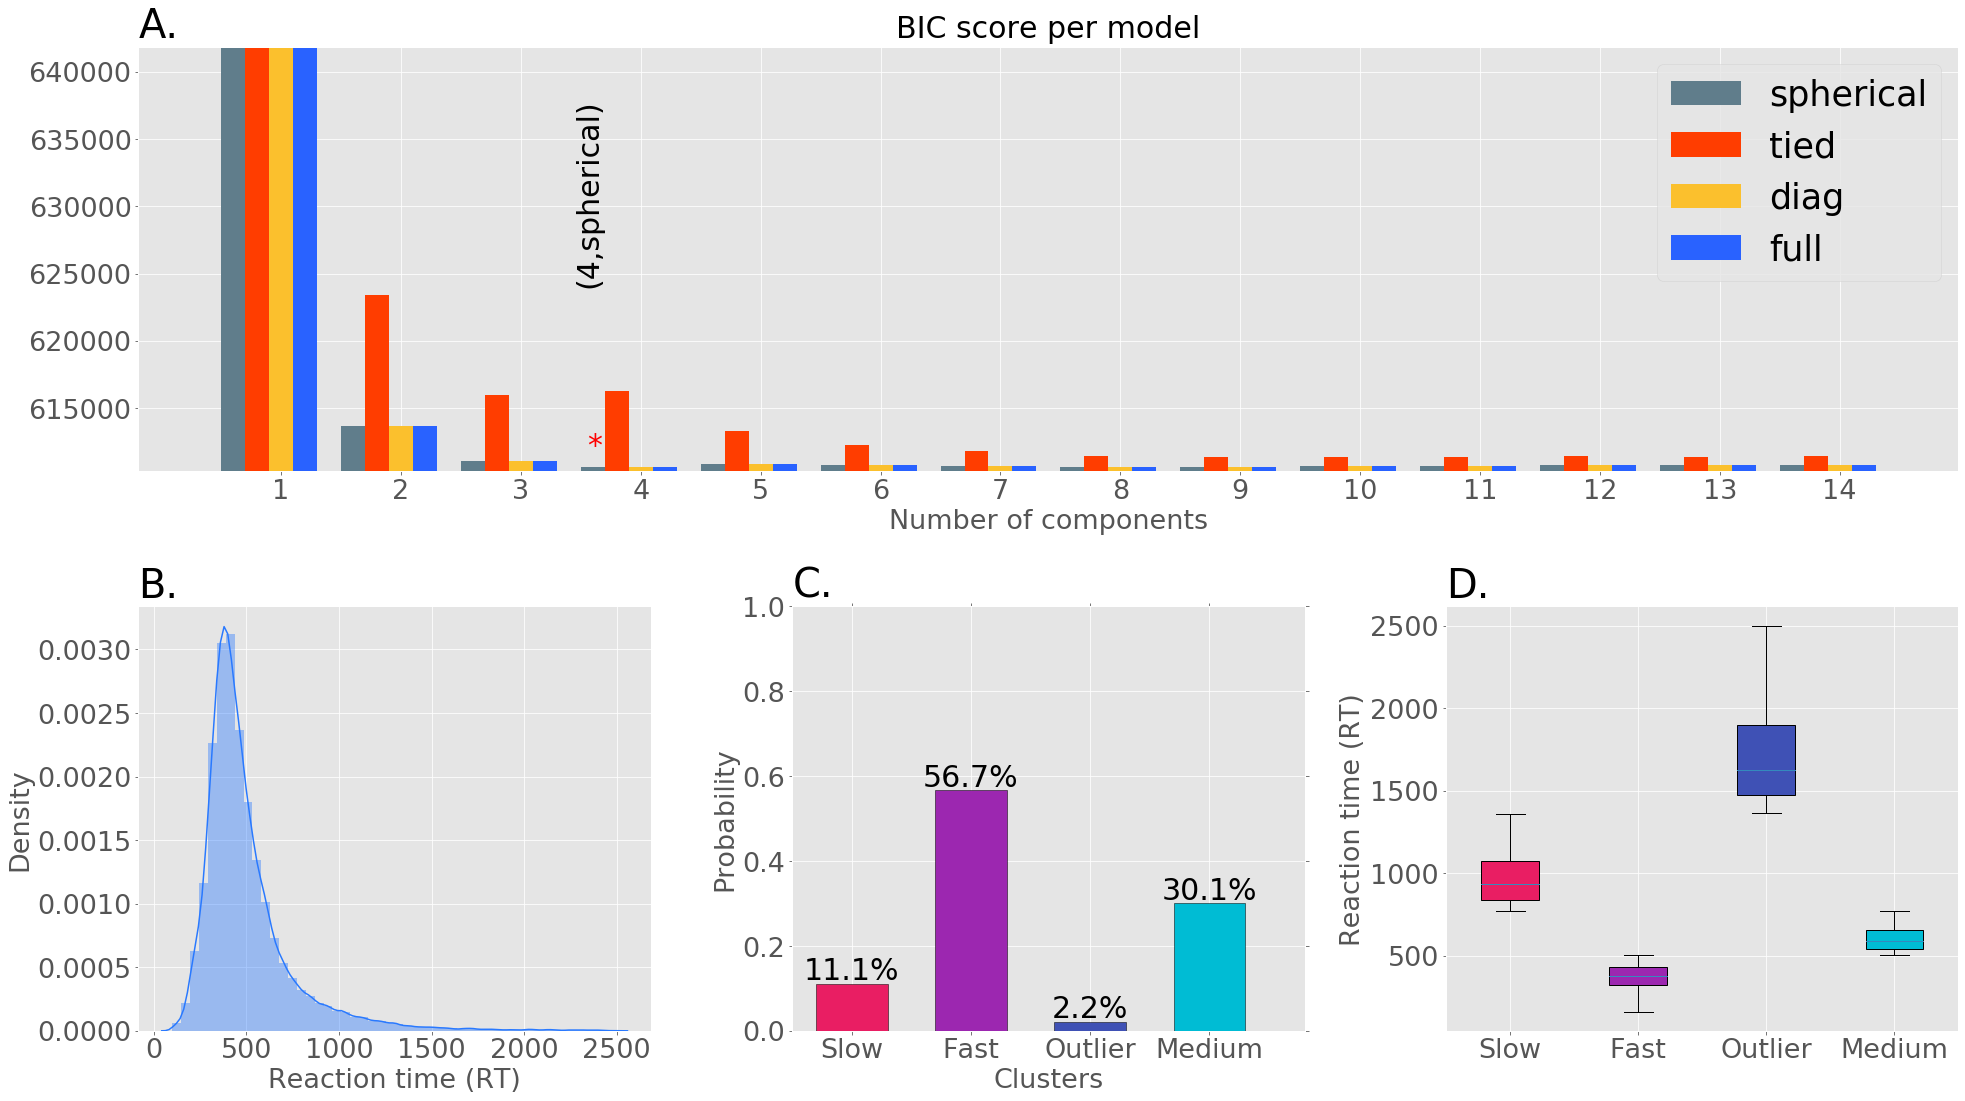
\includegraphics[width=\columnwidth]{Images/bic_gmm_optimization}}
\caption[Clustering of RT data.]{Clustering of RT data. A) BIC scores of models with different number of components and covariance type, the '*' denotes the model with the lowest BIC score. B) Original RT distribution. C) The probability of each RT clusters using the GMM with lowest BIC score. D) The RT range of each clusters (slow : 772 - 1360 ms, fast : 100 - 504 ms, outlier: 1364 - 2500 ms, medium: 506 - 770 ms}.
\label{rt_cluster}
\end{center}
\vskip -0.2in
\end{figure}

\textbf{Spatial-Spectral Representation:} As mentioned in section 1, we have opted to use bootstrapping to reduce noise in the EEG samples. We use the process of sampling trials with replacement in individual RT clusters and averaging them to generate ERPs. We sampled and averaged 50 trials at once in each RT cluster and repeated this process 500 times. The bootstrapping process of generating ERPs also works as a data augmentation step since we can generate more diverse samples by averaging different trials in each iteration. This process produced 62525 ERPs; we then compute the power spectral density (PSD) and band powers of these samples. We compute the bandpowers of three frequency bands: $\alpha$ (8-15 Hz), $\beta$ (16-31 Hz), and $\gamma$ (32–60 Hz). We used the built-in \emph{psd\_welch function}  provided in the open-source software package MNE-Python \cite{mne} to compute the PSDs. Next, we average the PSDs across $\alpha, \beta$ and $\gamma$ bands to acquire associated band power of the 64 spatial locations.

\begin{figure}[ht]
\vskip 0.2in
\begin{center}
\centerline{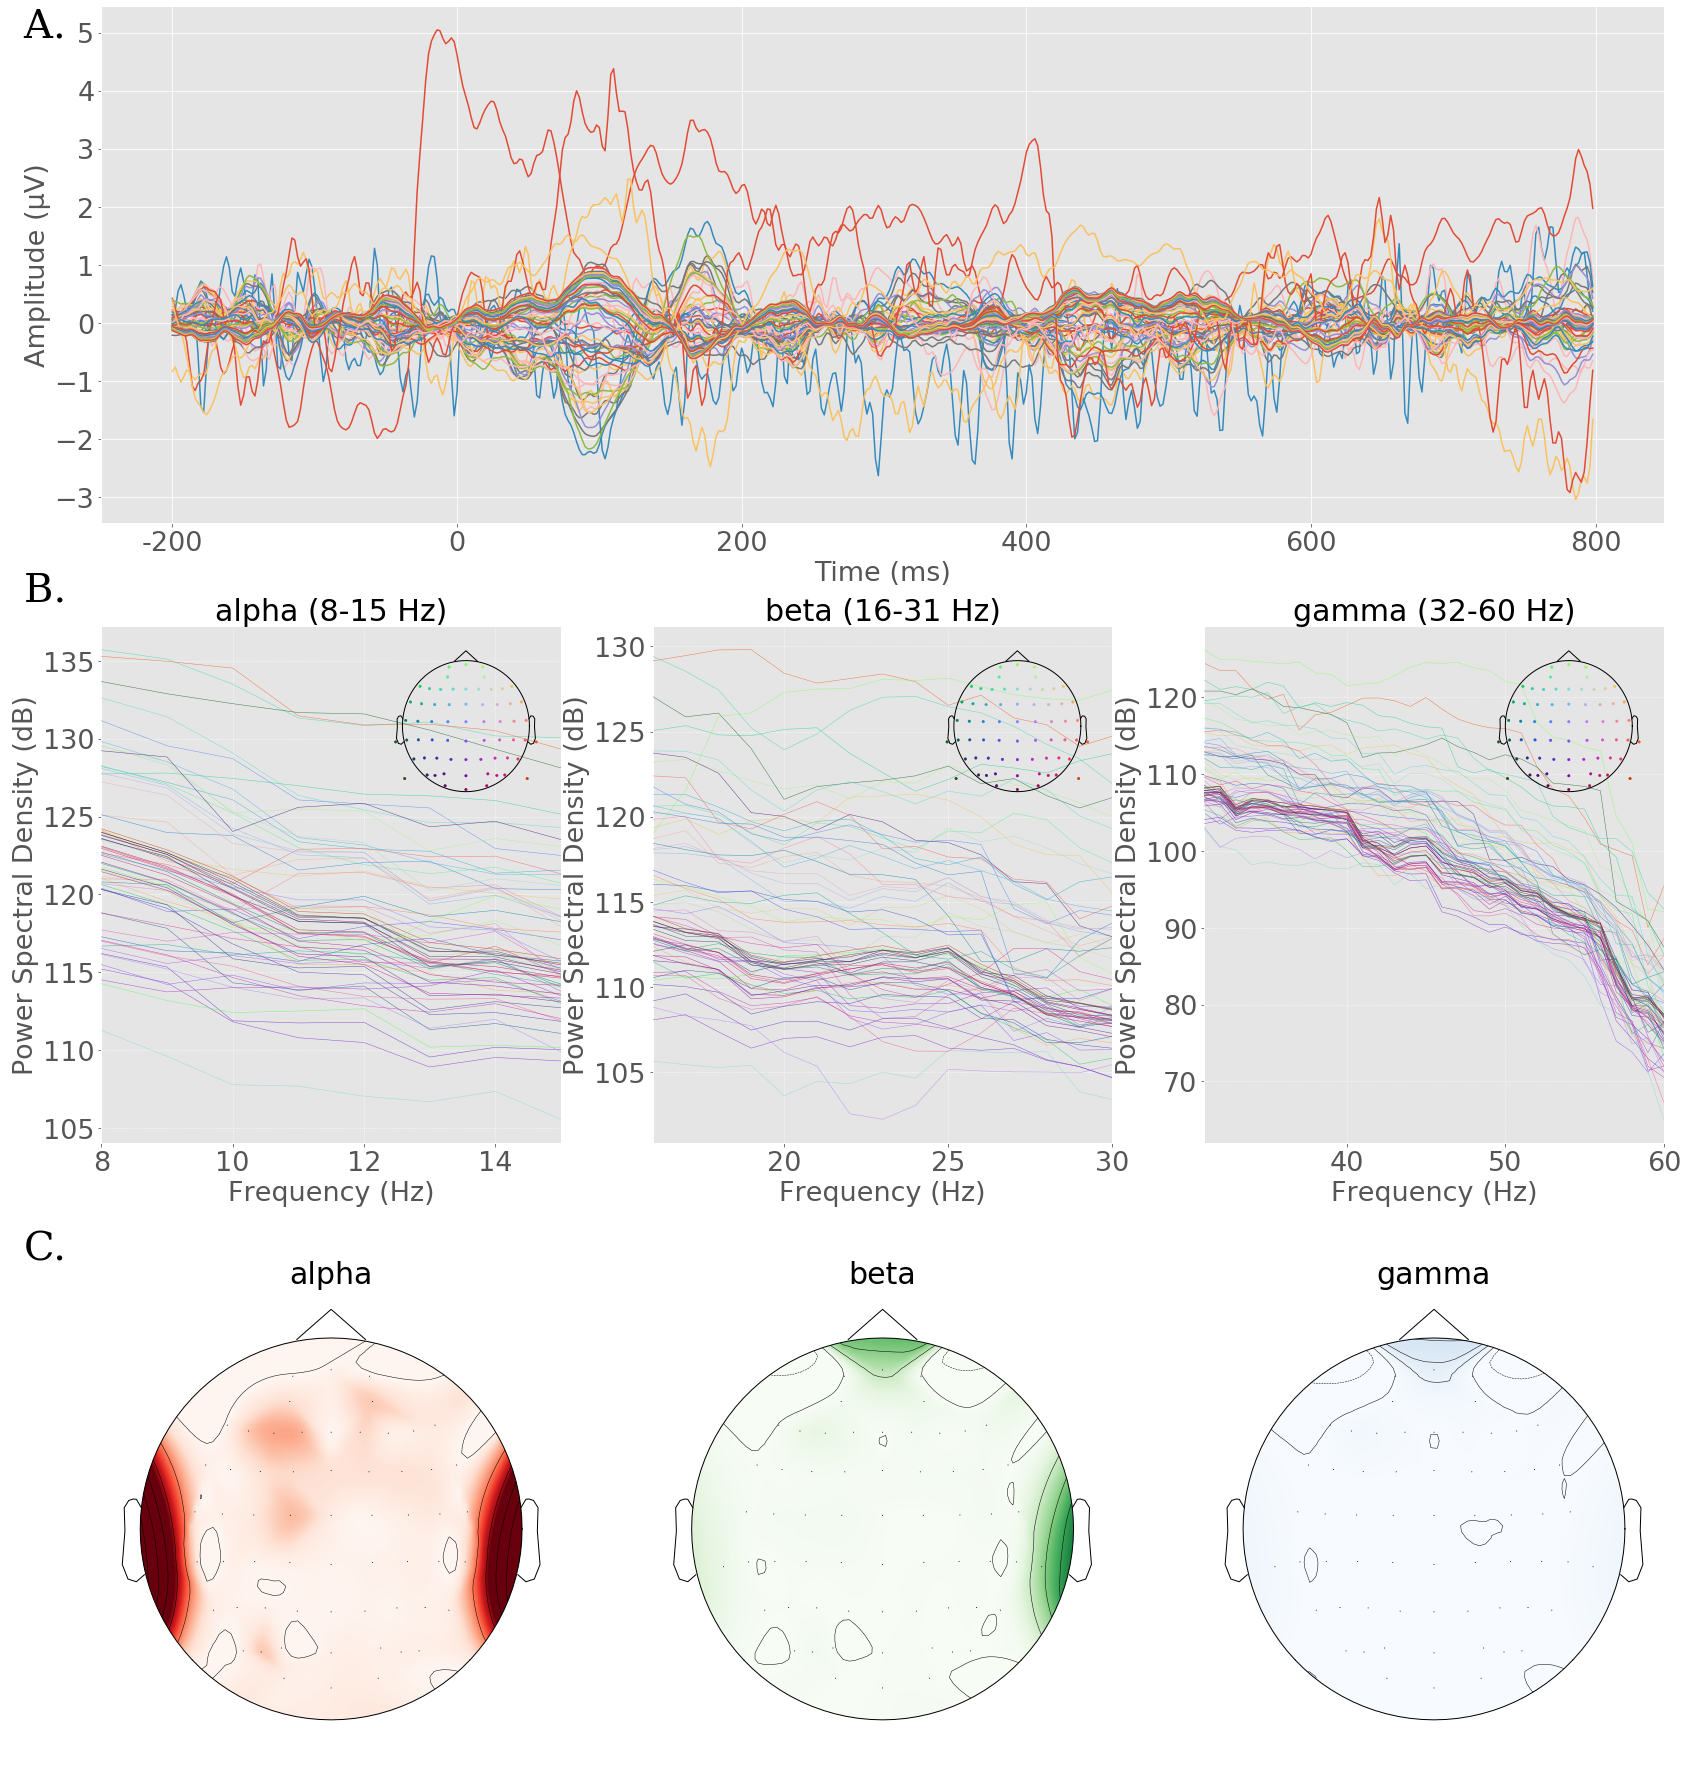
\includegraphics[width=\columnwidth]{Images/topomap_gen}}
\caption[Spatial-spectral topomap generation process]{A) ERP. B) PSDs of 64 spatial locations of $\alpha, \beta, \gamma$ frequency bands. C) Corresponding spatial topomaps of $\alpha, \beta, \gamma$ bands. D) Combined band power topomap through stacking of the $\alpha, \beta, \gamma$ topomaps.}
\label{topomap_gen}
\end{center}
\vskip -0.2in
\end{figure}

Figure \ref{topomap_gen} (A, B, C) depicts the band power calculation from the ERPs. We proceed to project these scaler band powers into a 2d topographical representation of the scalp known as topomap. The scaler band powers associated with each channel get mapped into the channels' location in the topomap and extrapolated (box) for crisp visual representation. We generate topomaps for the three-band powers $(\alpha, \beta, \gamma)$ individually, convert them to grayscale images, and stack them along the third dimension (RGB color channels). In this way, each of the bands gets represented through different color channels (see figure \ref{comine_band}). We used the \emph{plot\_topomap} from MNE-Python to generate the topomap images (size: $128 \times 128 \times 3$) from the average band powers.

\begin{figure}[ht]
\vskip 0.2in
\begin{center}
\centerline{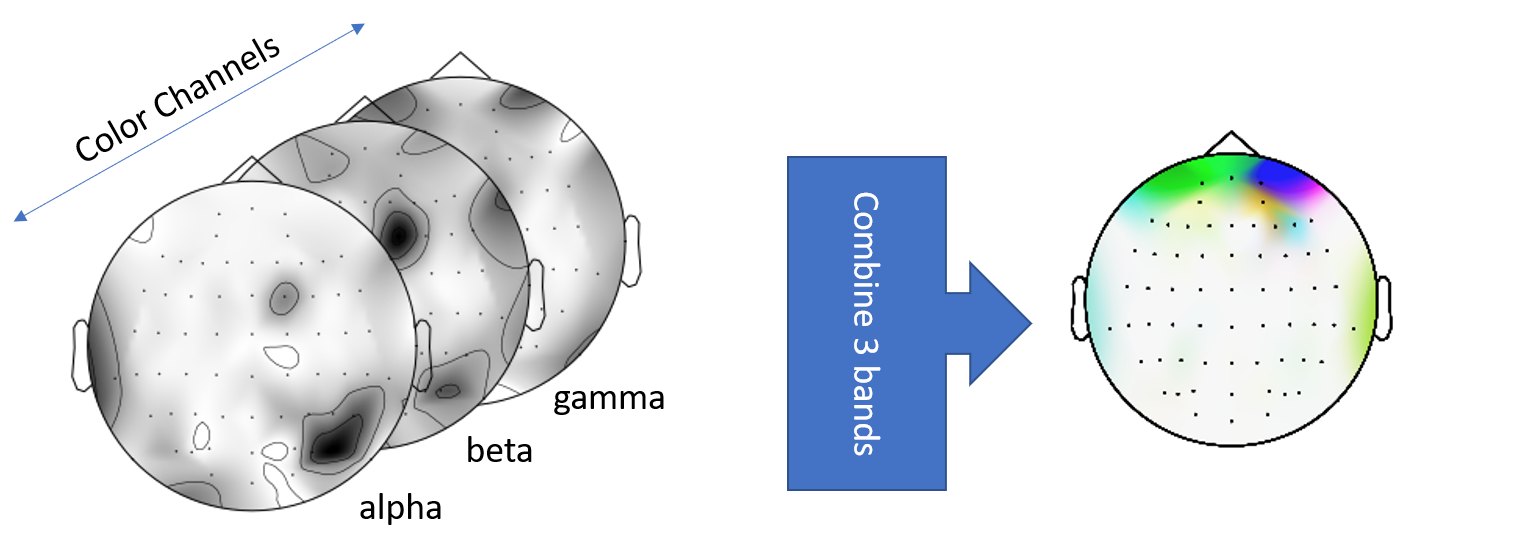
\includegraphics[width=\columnwidth]{Images/combine_bands}}
\caption[Spatial-spectral topomap generation process]{Combined band power topomap through stacking of the $\alpha, \beta, \gamma$ topomaps.}
\label{comine_band}
\end{center}
\vskip -0.2in
\end{figure}

\section{Modeling}

\begin{table*}[ht]
\caption{The hyperparameter optimized for CNNs with TPE}
\vskip 0.15in
\begin{center}
\begin{small}
    \begin{tabular}{ll}
      \textbf{Hyperparameter} & \textbf{Description} \\
      \hline
      $batch\_size$ & The batch size during training. \\
      $epochs$ & The number of epochs during training.  \\
      $first\_conv$ & The number of stacked convolution layers in the bottom of the network. \\
      $nb\_conv\_pool\_layers$ & The number of consecutive convolution and max-pool layers. \\
      $conv\_hiddn\_units\_mult$ & The number of filters in the 1st convolution layer ($40 \times mult$). \\
      $conv\_dropout\_drop\_proba$ &  The dropout probability of convolution filters. \\
      $residual$ & The number of residual layers, inspired by ResNet \cite{resnet}. \\
      $conv\_pool\_res\_start\_idx$ & The layer to start the residual connections. \\
      $fc\_units\_1\_mult$ & The number of neuron in the 1st fully connected (fc) layer ($750 \times mult$). \\
      $fc\_dropout\_drop\_proba$ & The dropout probability of neurons in the fully connected layers. \\
      $one\_more\_fc$ & The number of neurons in the 2nd layer of the fc layers ($750 \times mult$). \\
      $l2\_weight\_reg\_mult$ & The $l2$ regularization parameter ($\lambda = 0.0007 \times mult$). \\
      $lr\_rate\_mult$ & The learning rate parameter ($lr = 10 ^ {-5} \times mult$). \\
      $use\_BN$ & The use of batch normalization in convolution layers. \\
      $activation$ & The activation function in the convolution and fc layers. \\
      $optimizer$ & The optimization algorithm.
    \end{tabular}
\end{small}
\end{center}
\vskip -0.1in
\label{tab:tpe_var_Model}
\end{table*}

\textbf{Hyperparameter Optimization:} Using the bootstrap and average process, we generated 62525 ERP samples, which we converted to bandpower topomaps as described above. We used 46893 (75\%) samples for training and 15632 (25\%) samples for testing each model produced by the Bayesian hyperparameter optimization algorithm. We optimize the architecture and the general hyperparameters (e.g., batch size, epochs, learning rate) of CNN using TPE; table \ref{tab:tpe_var_Model} describes the hyperparameters optimized by TPE. We utilized Adam \cite{adam}, Nadam \cite{nadam} and RMSprop as the optimizers (learning algorithm) and ReLU \cite{relu, relu_2} or ELU \cite{elu} as activation functions during TPE optimization of Models. In the convolution layers, each layer contains twice the number of filters as the previous layer. If there are more than four layers, then the number of filters on each layer is iteratively increased with a constant value (the initial number of filters chosen by TPE). The kernel size of filters in convolution layers and residual layers are fixed ($3 \times 3$) with single strides (1, 1). The pooling size in max-pooling layers after convolution layers is also fixed ($2 \times 2$) with single strides (1, 1). We ran 35 trials of the TPE optimization to find the best hyperparameters of our CNN model. Figure \ref{test_acc_tpe} shows the test accuracy of each model generated by the TPE algorithm. We implemented the TPE algorithm for optimizing CNN using the open-source library hyperopt \cite{hyperopt}, and Keras \cite{keras}.

\begin{figure}[ht]
\vskip 0.2in
\begin{center}
\centerline{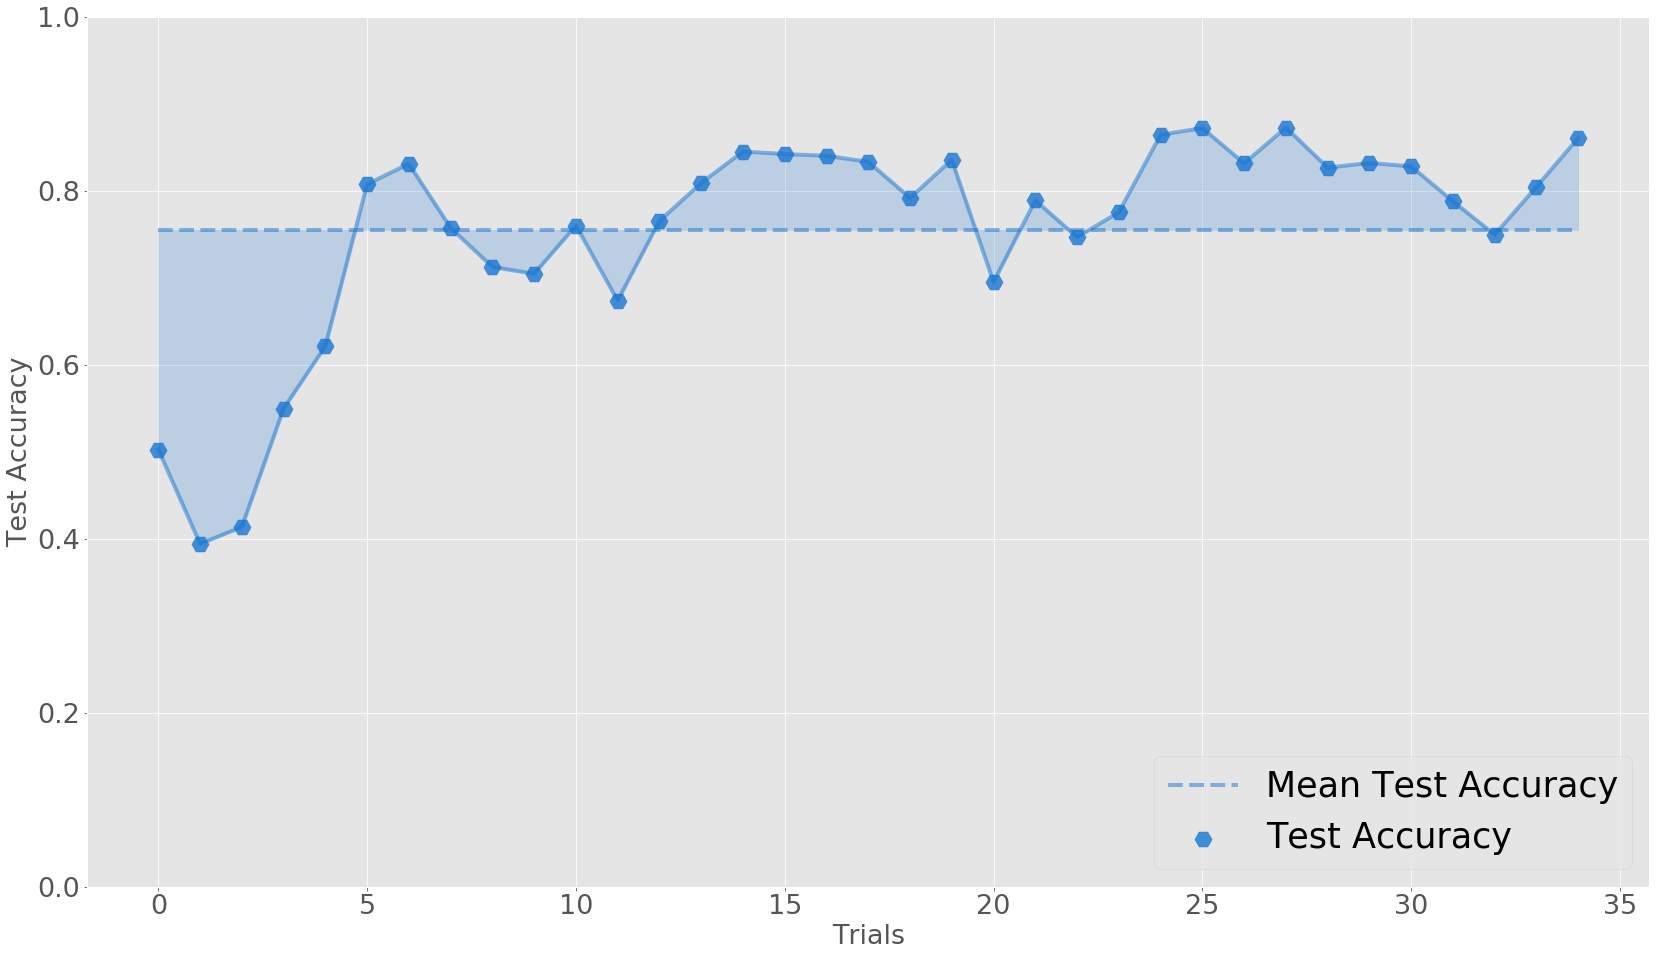
\includegraphics[width=\columnwidth]{Images/spsm_test_acc}}
\caption[Accuracy and loss curve of the best model]{Test accuracy of each models during the steps of hyperparameter optimization}
\end{center}
\vskip -0.2in
\label{test_acc_tpe}
\end{figure}

\textbf{Performance:} In this section, we evaluate our best CNN model (Model-10) of CP behavior. Among the 35 CNN models generated by the TPE algorithm, the mean test accuracy was 75.52\%, with the best performing model achieving an accuracy of 87.28\%. Figure \ref{acc_loss_best_model} shows our best model's loss and accuracy curve during the training session. We achieved an average (macro) of 87.70\% precision, 87.95\% recall, and 87.79\% f1-score, suggesting effective learning of neural patterns of different CP behavior. The slow, fast, and medium RTs achieved an average class probability score of 95\%, 93\%, and 92\%, respectively. The slow RT class was classified more accurately (precision: 89.63\%, recall: 91.4\% and f1-score: 90.52\%) compared to the other RT classes. Figure \ref{best_pr_cfm} shows the one vs. all precision-recall curve (PR curve), normalized and non-normalized confusion matrices. The area under the PR curve for the three RT categories (slow: 0.97, fast: 0.95, med: 0.94) suggests that the model can determine each category and distinguish between them skillfully. Table \ref{comparison} shows the performance comparison of the ten best models generated in the hyperparameter optimization process.

\begin{table*}[h]
        \caption{Performance comparison of 10 best CNN models generated by the TPE optimization algorithm.}
        \vskip 0.15in
        \begin{center}
        \begin{small}
        \begin{sc}
        \begin{tabular}{c | c | c | c | c }
        \textbf{Model} & \textbf{Precision} & \textbf{Recall} & \textbf{F1 Score} & \textbf{Accuracy} \\
        \hline
        Model-1 & 82.96\% & 84.80\% & 83.59\% & 83.22\% \\
        Model-2 & 84.25\% & 84.22\% & 84.05\% & 83.35\% \\
        Model-3 & 84.23\% & 84.25\% & 84.16\% & 83.58\% \\
        Model-4 & 84.97\% & 84.46\% & 84.69\% & 84.05\% \\
        Model-5 & 84.43\% & 85.29\% & 84.83\% & 84.25\% \\
        Model-6 & 84.90\% & 85.24\% & 85.01\% & 84.53\% \\
        Model-7 & 86.21\% & 87.10\% & 86.60\% & 86.09\% \\
        Model-8 & 87.12\% & 87.02\% & 87.07\% & 86.46\% \\
        Model-9 & 87.54\% & 88.03\% & 87.75\% & 87.24\% \\
        Model-10 (best) & 87.70\% & 87.95\% & 87.79\% & 87.28\% \\
       \end{tabular}
     \end{sc}
     \end{small}
     \end{center}
     \vskip -0.1in
     \label{comparison}
   \end{table*}

\begin{figure}[ht]
\vskip 0.2in
\begin{center}
\centerline{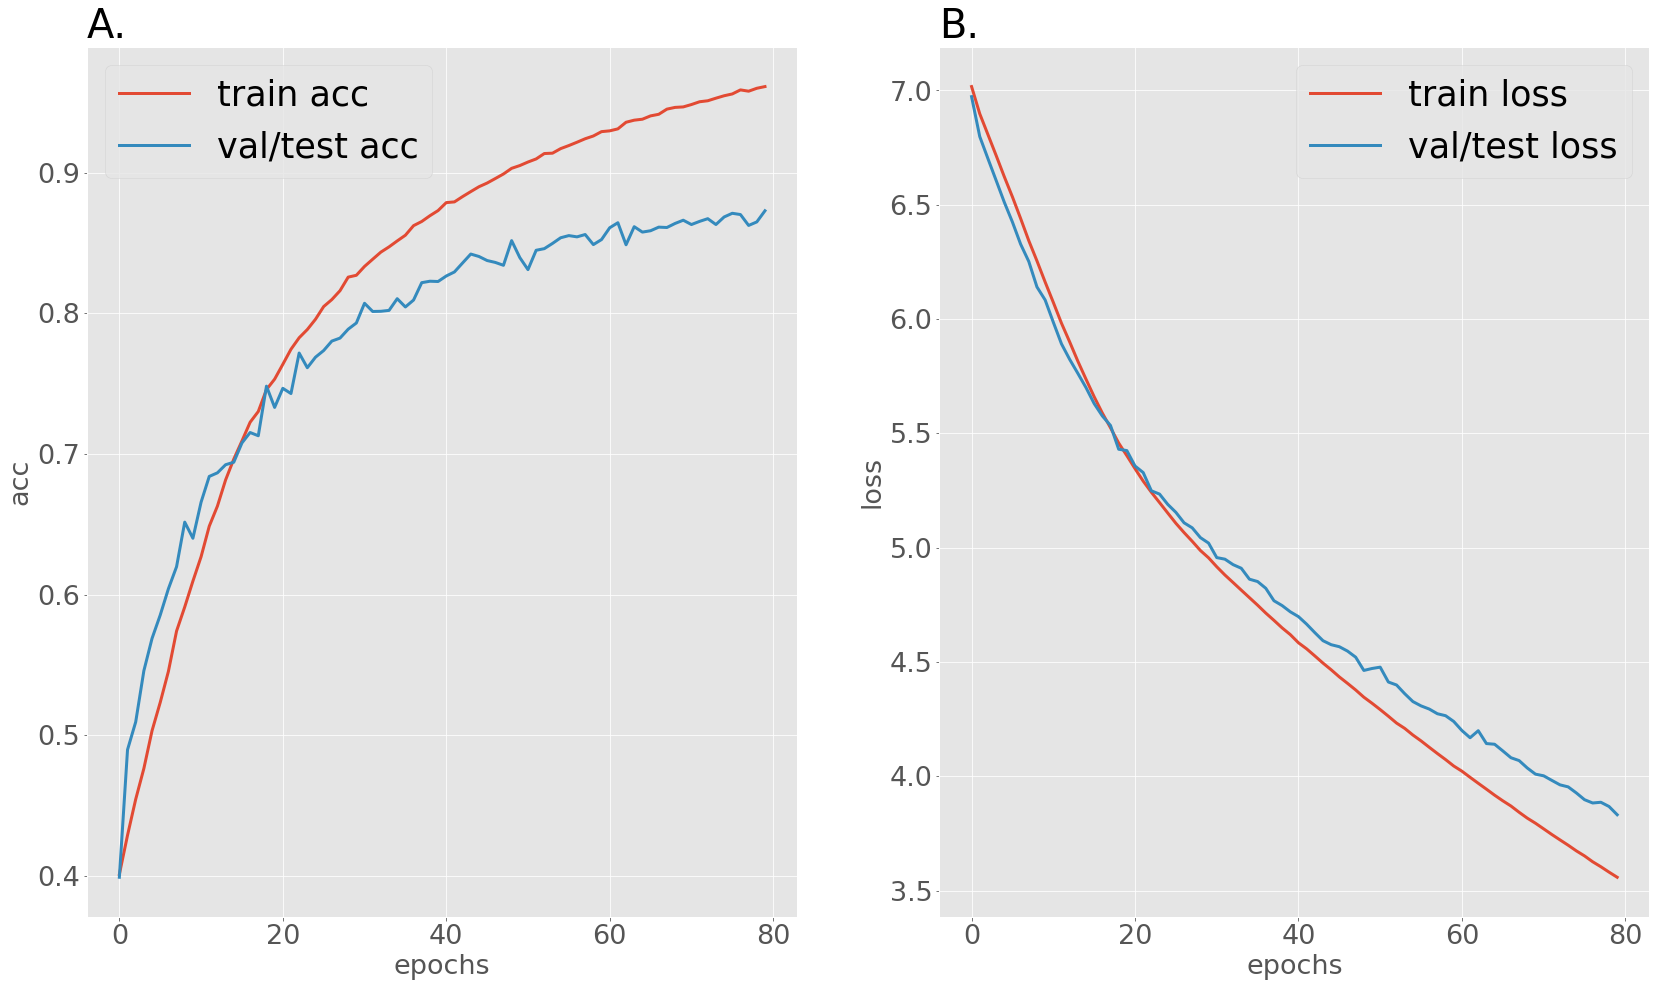
\includegraphics[width=\columnwidth]{Images/acc_loss_best_model}}
\caption[Accuracy and loss curve of the best model]{Accuracy (A) and loss curve (B) of best performing CNN during training.}
\end{center}
\vskip -0.2in
\label{acc_loss_best_model}
\end{figure}

\begin{figure}[ht]
\vskip 0.2in
\begin{center}
\centerline{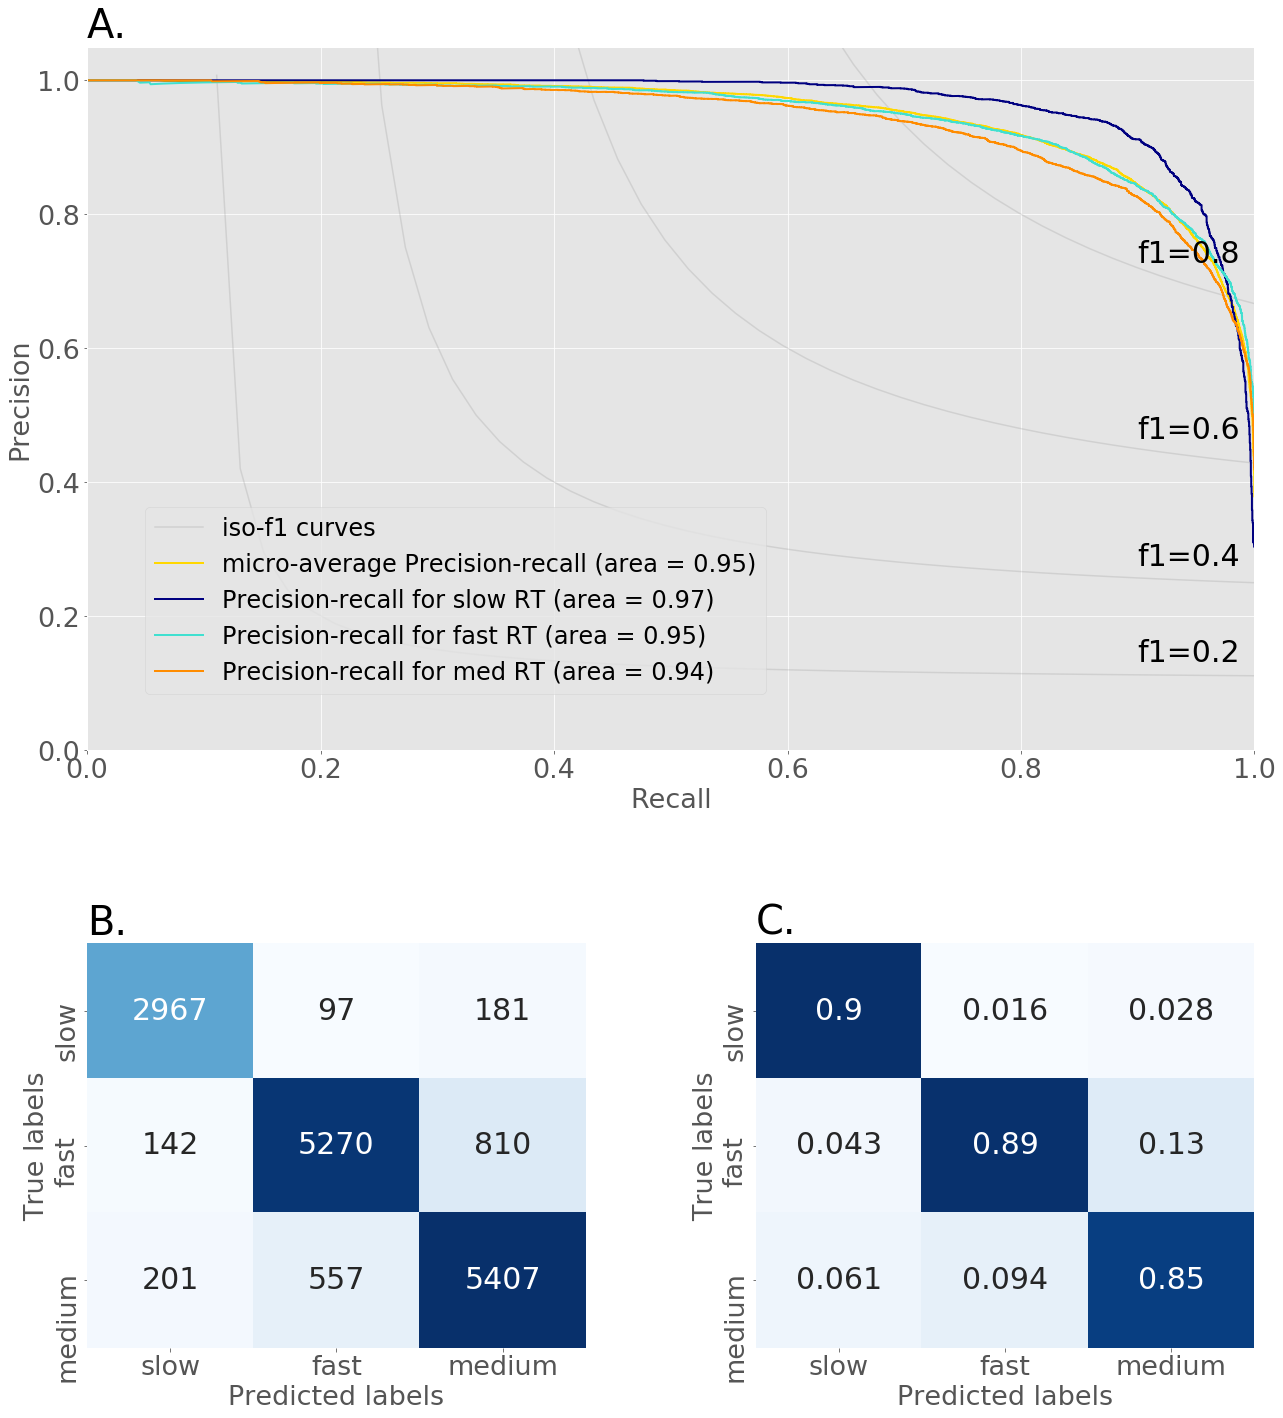
\includegraphics[width=\columnwidth]{Images/best_pr_cfm}}
\caption[Accuracy and loss curve of the best model]{A) Precision-recall curve B) Confusion matrix C) Normalized confusion matrix}
\end{center}
\vskip -0.2in
\label{best_pr_cfm}
\end{figure}

\section{Learned Representation}

\textbf{GradCAM and Guided-GradCAM:} In this section, we present the learned representation of Model-10 (see table \ref{comparison}), which is our best CP behavior model. We use GradCAM and Guided-GradCAM visualization to get an insight into the learned spatial-spectral features of our best CNN. GradCAM is a visual interpretation tool that depicts a coarse localization map of an image detected by CNN w.r.t a class or label \cite{gradcam}. GradCAM uses gradients of a class flowing into the final convolution layer to produce such visualizations. Guided-GradCAM is another class discriminative activation map that combines Guided-Backpropagation \cite{allconvnet} with GradCAM to produce channel-wise activation maps. Figure \ref{ggbp} illustrates some GradCAM and Guided-GradCAM visualization of the learned features by CNN. As mentioned in section 1, visualization alone is not enough to infer a models' learned representation. Therefore, we have taken the activation values from the Guided-GradCAM output to measure the learned representation of the CNN. Since we have 64 spatial locations in our input topomaps, we need 64 activation values to quantify the learned features of CNN. We extract the activation values surrounding the neighborhood of each of these spatial locations by applying a median filter ($20 \times 20$). Figure \ref{ggbp_cal} show the channel (band) wise extraction of activation values through median filters.

\begin{figure}[ht]
\vskip 0.2in
\begin{center}
\centerline{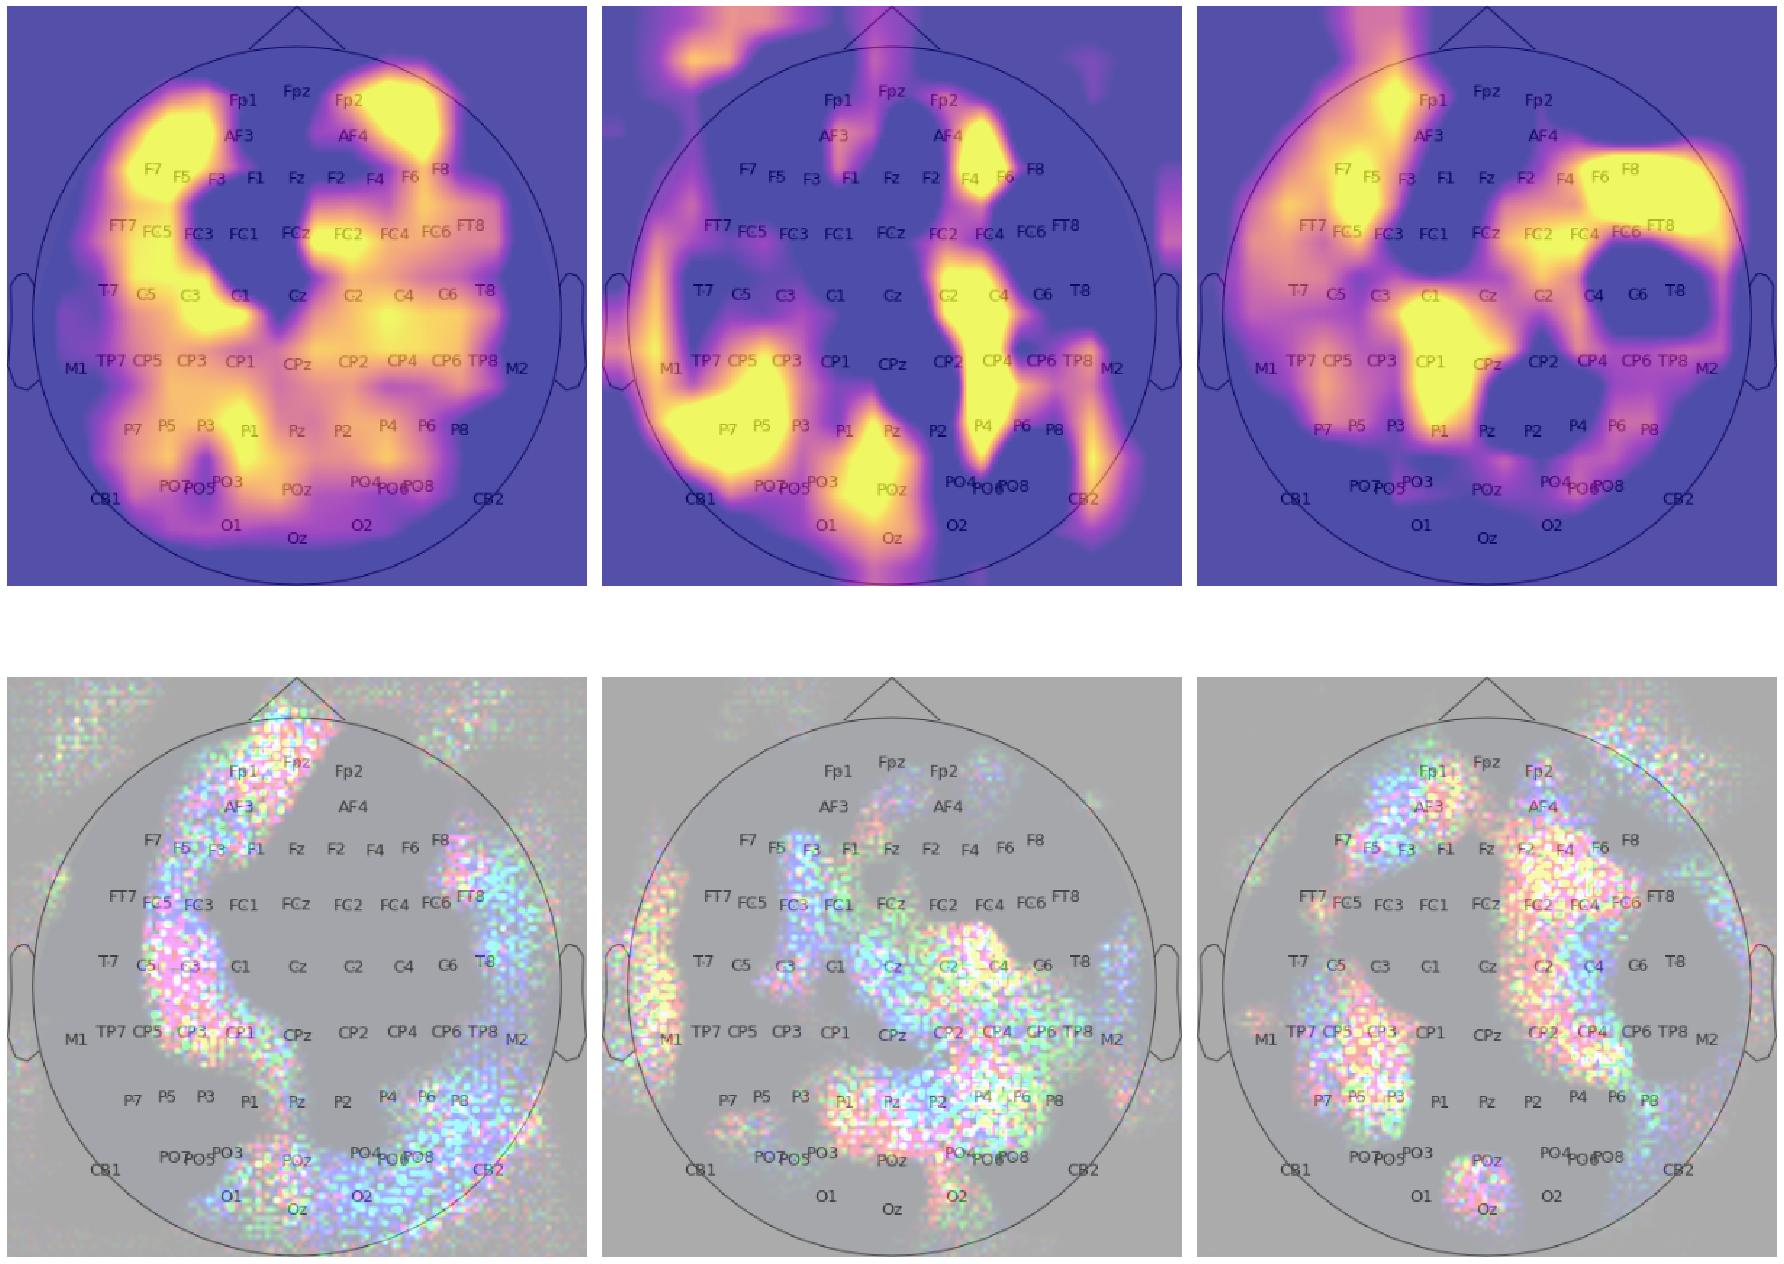
\includegraphics[width=\columnwidth]{Images/sample_gradcam_ggbp}}
\caption[Activation maps from GradCAM and Guided-GradCAM]{Activation maps from GradCAM (1st) and Guided-GradCAM (2nd)}
\end{center}
\vskip -0.2in
\label{ggbp}
\end{figure}

\begin{figure}[ht]
\vskip 0.2in
\begin{center}
\centerline{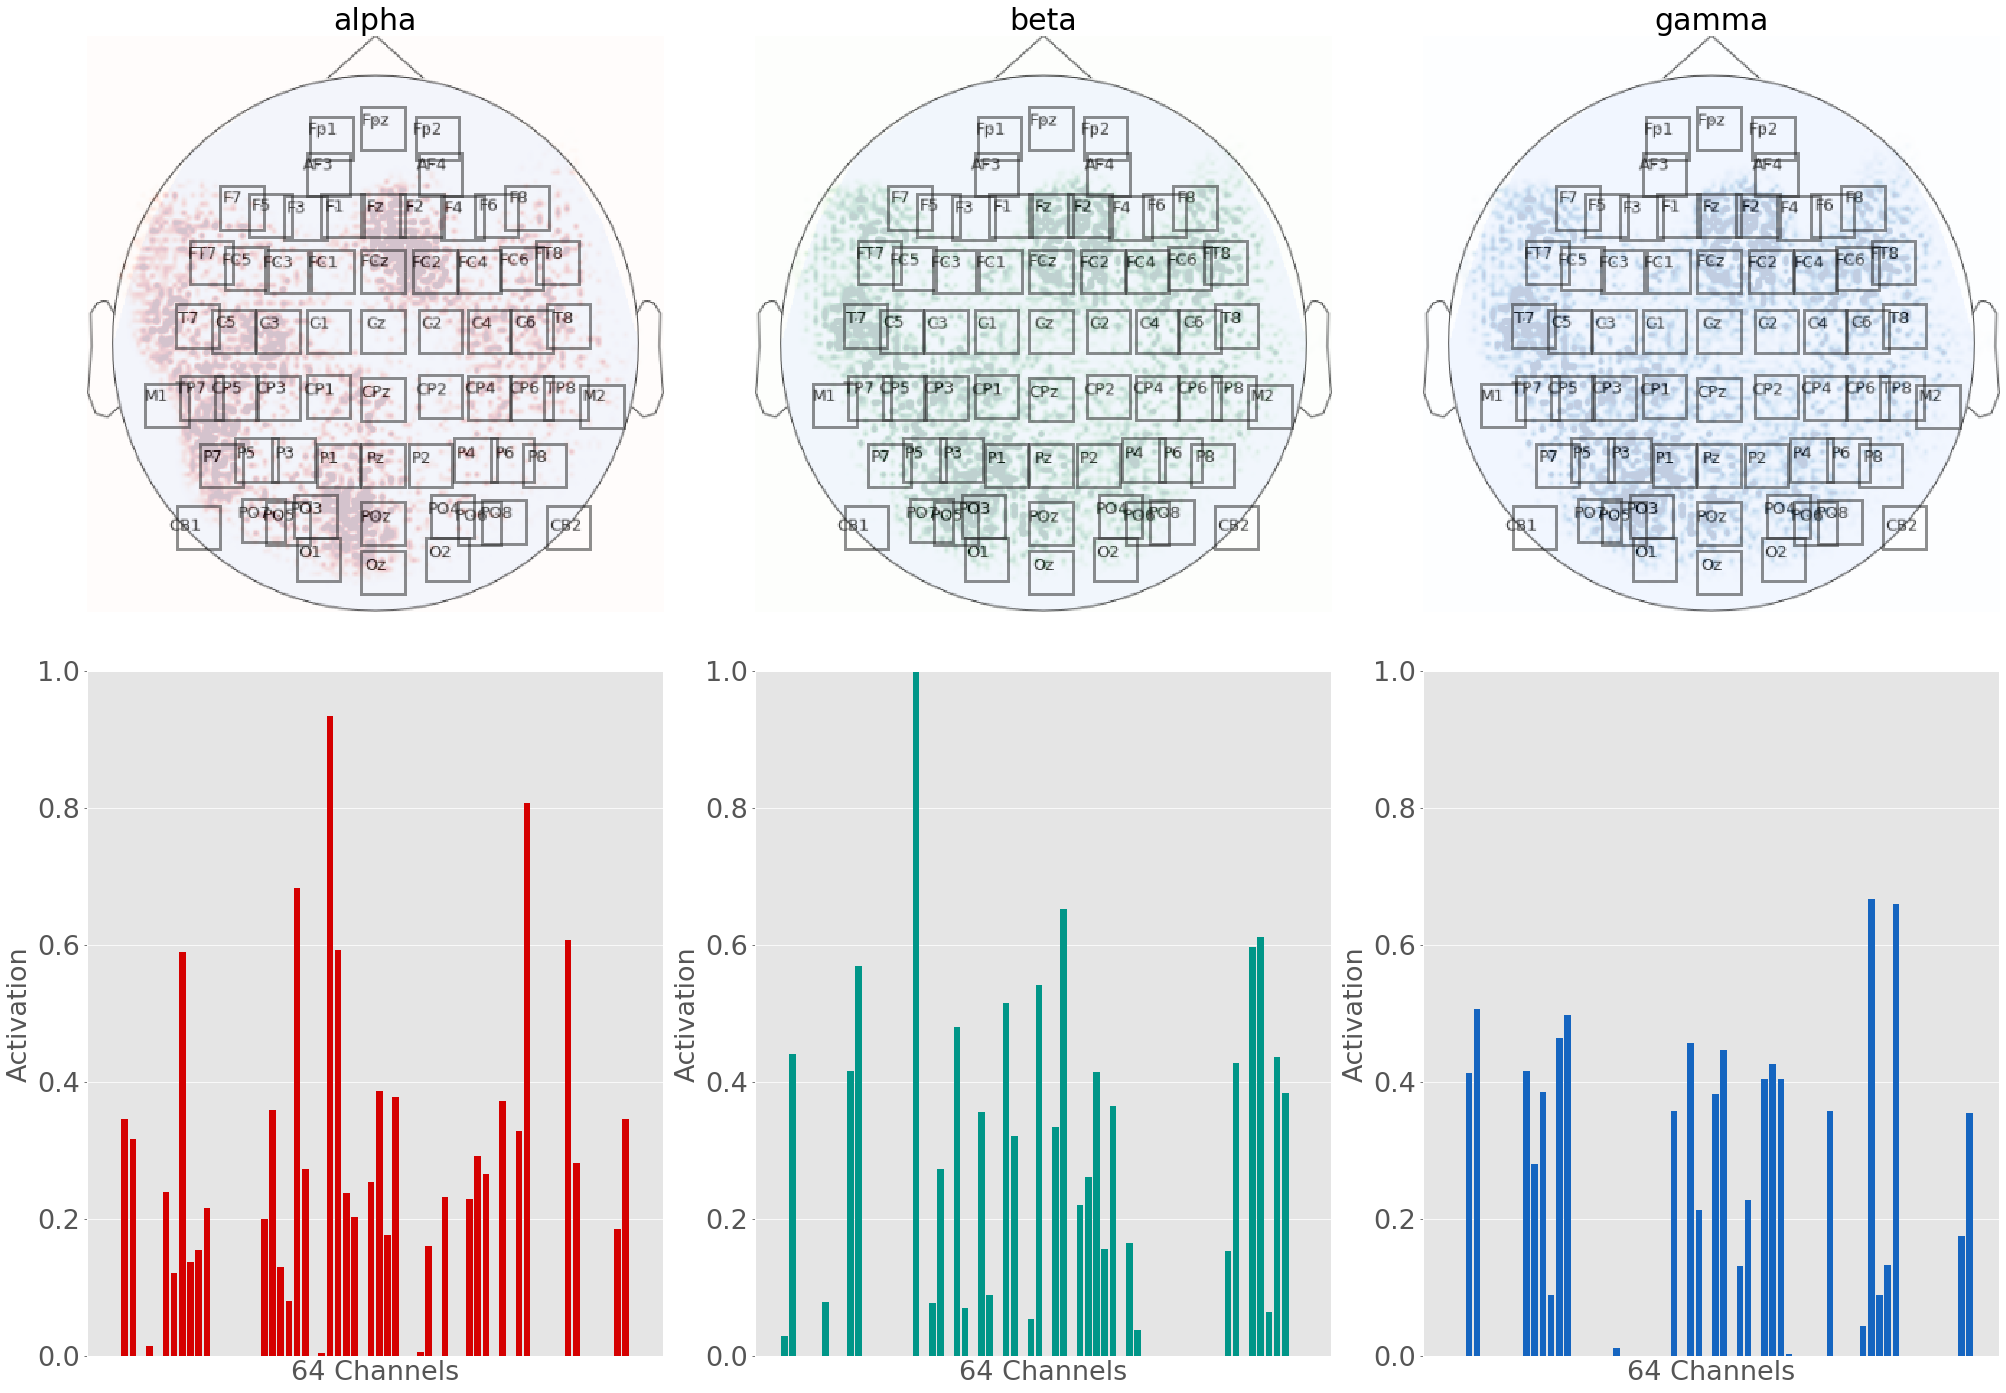
\includegraphics[width=\columnwidth]{Images/saliency_score_cal_ggbp}}
\caption[Activation maps from GradCAM and Guided-GradCAM]{Band-wise activation value extraction from Guided-GradCAM outputs, the 1st row show the median filters on the 64 spatial location on each frequency bands, the 2nd row shows the extracted median activation values from the surroundings of those locations.}
\end{center}
\vskip -0.2in
\label{ggbp_cal}
\end{figure}

\textbf{Statistical Analysis:} We apply ANOVA analysis on the activation values to observe the significance of learned spatial-spectral representations between the RT categories. The analysis shows a significant difference in spatial activation between the bands ($p = 2.2e^{-16}$), validating that our spatial-spectral representation was accurate. It also confirms that our model was able to capture the different regional operations of individual bands. We also find different band activation between the RT categories ($p = 0.024$), implying that our model effectively learned these frequency bands' role in CP tasks. Another observation from the analysis is that there is significant ($p = 0.0056$) variation within the RT categories, further confirming that the neural process underlying speech categorization speed is subject to high variation. Overall, the ANOVA analysis showed that our best model was able to effectively capture the variable neural factors contributing to speech categorization speed. To infer from the learned representation, we have conducted Tukey HSD tests on the activation values. We focus on finding the spatial and spectral factors that contribute to different decision speed in CP.


\textbf{Neural Correlates of CP Behavior}: Auditory categorization in the human brain is revealed to use a distributed frontal-temporal-parietal network by contemporary EEG studies \cite{plasticity_sp, language_sp, Al_Fahad_2020}. The canonical language processing is left hemisphere (LH) predominantly. However, through analysis of the activations from Guided-GradCAM, we find that right hemisphere (RH) engagement is responsible for decoding RT of categorical speech processing. Especially, frontal regions in RH (F8, F6, FC2, FC4, FC6) are significant in mapping speech to the behavioral responses. \cite{RH_IFG1, RH_IFG2} found through fMRI experiments that right inferior frontal gyrus (IFG) activation is responsible for attentional control and detection of task-relevant cues. We have similar findings as to the fast and medium RT groups show more importance in the F6, F8, FC6, FC8 spatial locations (presumably IFG), implying more attentional power in speech categorization decision (see figure \ref{overall_sp_saliency}). The Tukey HSD test on the spatial activations revealed that CP1 and P2 locations significantly discriminate the slow RTs from the other two classes. CP1 and P2 are part of a distributed activation that we observe across the parietal lobe (in both hemispheres for slow and med RTs, predominantly in RH for fast RTs). The parietal lobe has the function of managing short-term memory and retrieving encoded verbal material during speech perception \cite{parietal}. Therefore, it is evident from this finding that delay in retrieval of encoded materials is also a factor contributing to slow RTs.

\begin{figure}[ht]
\vskip 0.2in
\begin{center}
\centerline{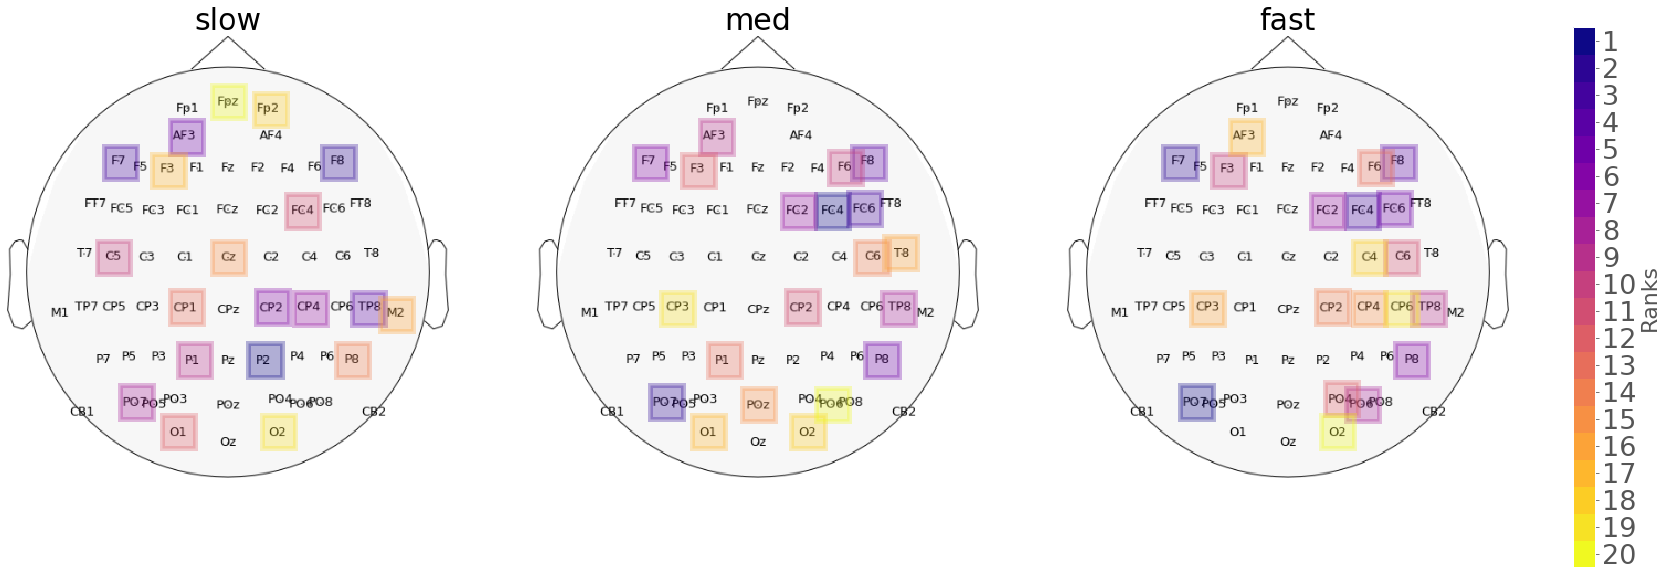
\includegraphics[width=\columnwidth]{Images/overall_class_discriminative_spatial_saliency}}
\caption[Ranked spatial features by activation values]{Top 20 ranked spatial features by mean activation values, the features are ranked by taking the mean of actiavtion across all test samples of a RT class. }
\end{center}
\vskip -0.2in
\label{overall_sp_saliency}
\end{figure}

In terms of perceptual encoding of speech, we also find our spatial results to be coherent as \cite{Bidelman2016FunctionalCI} found that audio stimuli of lower SNR cause increased engagement of primary auditory cortex (PAC) and IFG in RH. Participants in our experiment predominantly reacted faster when given clear tokens (TK 1, 2, 4, 5) than the ambiguous one (TK. 3) (see figure \ref{RT_var}), which explains the functional lateralization of RH. In slower RT, we find more distributed region activations, especially lateralization of the LH, and lesser activation in frontal regions of RH. The lateralization of LH suggests increased use of language processing units, whereas low activation in the distributed frontal regions of RH implies a lack of attentional control.

\begin{figure}[ht]
\vskip 0.2in
\begin{center}
\centerline{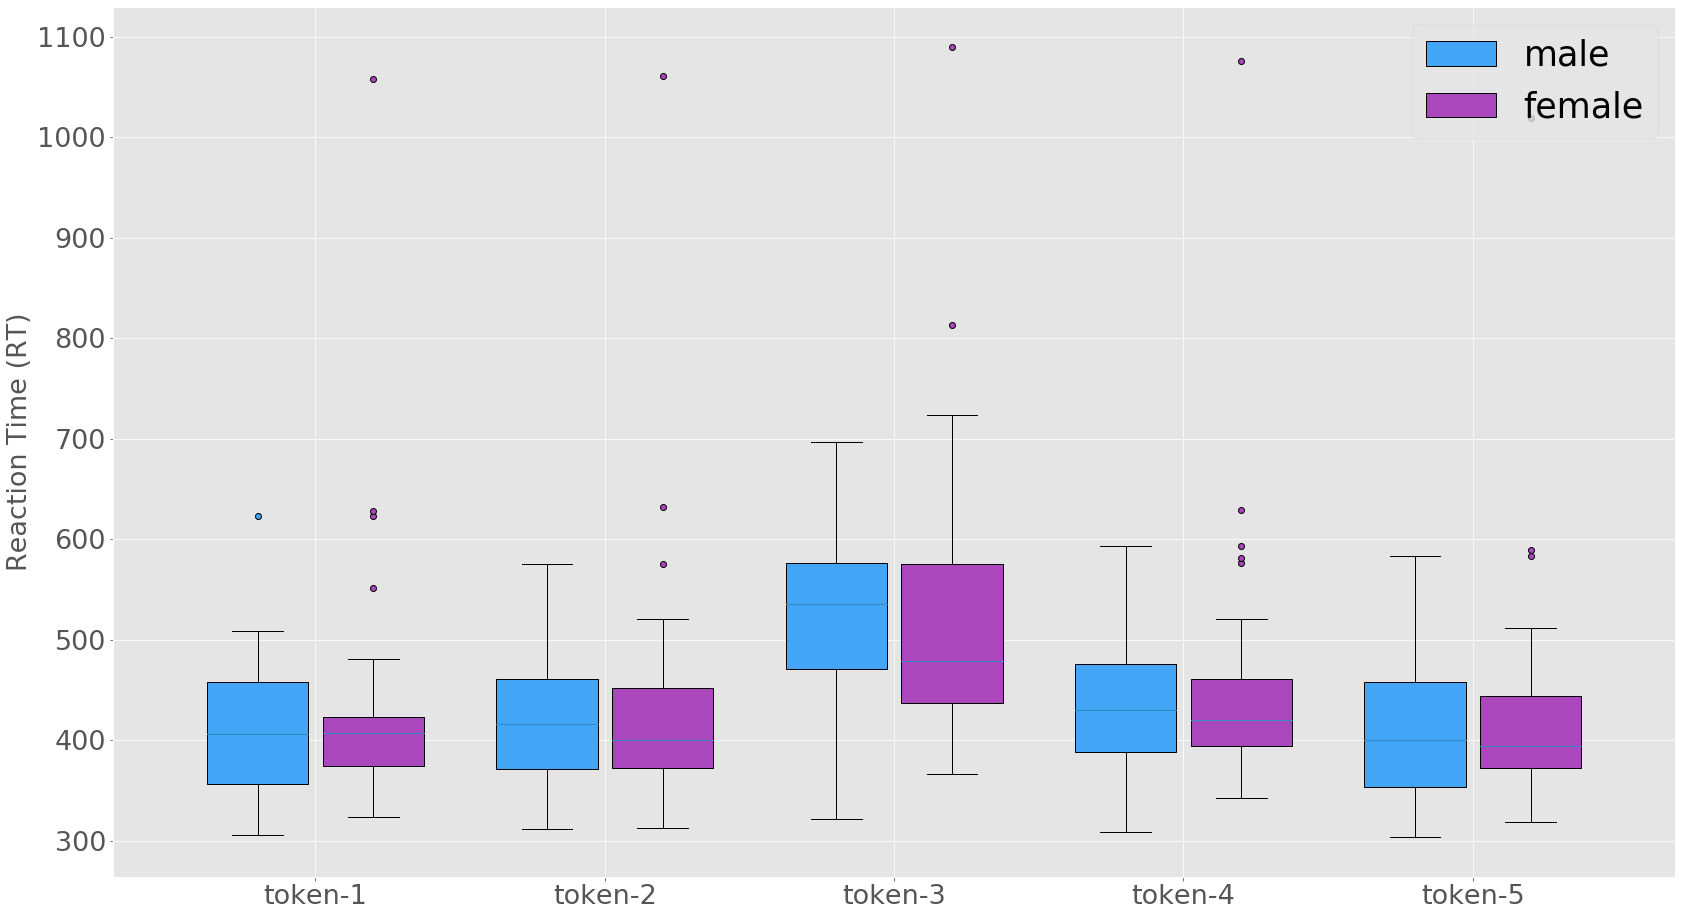
\includegraphics[width=\columnwidth]{Images/RT_var}}
\caption[Ranked spatial features by activation values]{Variation of RTs across tokens}
\end{center}
\vskip -0.2in
\label{RT_var}
\end{figure}

We assess through pairwise Tukey HSD test that $\gamma$ band significantly distinguishes between the fast-med ($p = 0.0069$) and med-slow ($p = 0.0098$) group. $\gamma$ band also achieved the highest mean activation (0.0093) and is thus more predictive of participants' decision time. The significance of the $\gamma$ band is coherent with the recent study of \cite{Mahmud2020} where $\gamma$ band modulations are found to be more correlated with listeners' behavioral CP. $\gamma$ is found to be responsible for auditory object construction \cite{obj_con_gamma} and local network synchronization \cite{net_gamma1, net_gamma2, net_gamma3}. Since we have the effect of musical training in our participants, the saliency of the $\gamma$ band might also reflect experience-dependent enhancement in CP. $\gamma$ band is found to be a reflection of enhancement in individuals' CP dictated by their musical experience.


\section{Conclusion}

In the prescribed study, we have demonstrated a novel way to decode neural activities dictating individuals' RT from EEG data using CNN. We have found the efficacy of our approach by further confirming several supporting hypotheses of speech categorization behavior. Although the science of interpreting CNN models is still in its early steps, we show that existing tools like GradCAM and Guided-GradCAM can be used to explain the neurological properties of behavioral auditory CP. Our proposed process could be extended to decode other cognitive functions from EEG data.
% Acknowledgements should only appear in the accepted version.
\section*{Acknowledgements}

\textbf{Do not} include acknowledgements in the initial version of
the paper submitted for blind review.

If a paper is accepted, the final camera-ready version can (and
probably should) include acknowledgements. In this case, please
place such acknowledgements in an unnumbered section at the
end of the paper. Typically, this will include thanks to reviewers
who gave useful comments, to colleagues who contributed to the ideas,
and to funding agencies and corporate sponsors that provided financial
support.


% In the unusual situation where you want a paper to appear in the
% references without citing it in the main text, use \nocite
\nocite{langley00}

\bibliography{references}
\bibliographystyle{icml2021}


%%%%%%%%%%%%%%%%%%%%%%%%%%%%%%%%%%%%%%%%%%%%%%%%%%%%%%%%%%%%%%%%%%%%%%%%%%%%%%%
%%%%%%%%%%%%%%%%%%%%%%%%%%%%%%%%%%%%%%%%%%%%%%%%%%%%%%%%%%%%%%%%%%%%%%%%%%%%%%%
% DELETE THIS PART. DO NOT PLACE CONTENT AFTER THE REFERENCES!
%%%%%%%%%%%%%%%%%%%%%%%%%%%%%%%%%%%%%%%%%%%%%%%%%%%%%%%%%%%%%%%%%%%%%%%%%%%%%%%
%%%%%%%%%%%%%%%%%%%%%%%%%%%%%%%%%%%%%%%%%%%%%%%%%%%%%%%%%%%%%%%%%%%%%%%%%%%%%%%
\appendix
\section{Do \emph{not} have an appendix here}

\textbf{\emph{Do not put content after the references.}}
%
Put anything that you might normally include after the references in a separate
supplementary file.

We recommend that you build supplementary material in a separate document.
If you must create one PDF and cut it up, please be careful to use a tool that
doesn't alter the margins, and that doesn't aggressively rewrite the PDF file.
pdftk usually works fine.

\textbf{Please do not use Apple's preview to cut off supplementary material.} In
previous years it has altered margins, and created headaches at the camera-ready
stage.
%%%%%%%%%%%%%%%%%%%%%%%%%%%%%%%%%%%%%%%%%%%%%%%%%%%%%%%%%%%%%%%%%%%%%%%%%%%%%%%
%%%%%%%%%%%%%%%%%%%%%%%%%%%%%%%%%%%%%%%%%%%%%%%%%%%%%%%%%%%%%%%%%%%%%%%%%%%%%%%


\end{document}


% This document was modified from the file originally made available by
% Pat Langley and Andrea Danyluk for ICML-2K. This version was created
% by Iain Murray in 2018, and modified by Alexandre Bouchard in
% 2019 and 2021. Previous contributors include Dan Roy, Lise Getoor and Tobias
% Scheffer, which was slightly modified from the 2010 version by
% Thorsten Joachims & Johannes Fuernkranz, slightly modified from the
% 2009 version by Kiri Wagstaff and Sam Roweis's 2008 version, which is
% slightly modified from Prasad Tadepalli's 2007 version which is a
% lightly changed version of the previous year's version by Andrew
% Moore, which was in turn edited from those of Kristian Kersting and
% Codrina Lauth. Alex Smola contributed to the algorithmic style files.
